% !TEX program = xelatex
\documentclass[a4paper]{article}
\usepackage{amsmath}
\usepackage{amsthm}
\usepackage[left=1.8cm,right=1.8cm,top=2.2cm,bottom=2.0cm]{geometry}
\usepackage{ctex}
\usepackage{enumerate}
\usepackage{fancyhdr}
\usepackage{xpatch}
\usepackage{graphicx} 
\usepackage{float} 
\usepackage{subfigure} 
\usepackage{amsfonts}
\usepackage{mathtools}
\usepackage{framed}
\usepackage{multicol}
\usepackage{minted}
\usepackage{amsmath}
\usepackage{hyperref}
\usepackage{tikz}
\usepackage{biblatex}
\addbibresource{10-discussion.bib}
\usetikzlibrary{automata,positioning}
\theoremstyle{definition}
\newtheorem*{solution*}{\textbf{Solution:}}
\newtheorem*{proof*}{\textbf{Proof:}}
\newtheorem{theorem}{Theorem}[subsection]
\newtheorem{definition}{Definition}[subsection]
\newtheorem{lemma}{Lemma}[subsection]
\makeatletter
\usepackage{listings}% http://ctan.org/pkg/listings
\lstset{
  basicstyle=\ttfamily\tiny,
  mathescape,
}
\AtBeginDocument{\xpatchcmd{\@thm}{\thm@headpunct{.}}{\thm@headpunct{}}{}{}}
\makeatother

\pagestyle{fancy}
\renewcommand{\baselinestretch}{1.15}

\usepackage{paralist}
\let\itemize\compactitem
\let\enditemize\endcompactitem
\let\enumerate\compactenum
\let\endenumerate\endcompactenum
\let\description\compactdesc
\let\enddescription\endcompactdesc

% shorten footnote rule
\xpatchcmd\footnoterule
  {.4\columnwidth}
  {1in}
  {}{\fail}

\title{CS 131 Compilers: Discussion 10: Static Analysis}
\author{\textbf{杨易为}~~\textbf{吴凌云}~~\textbf{樊雨鑫} \\ \texttt{ \{yangyw,wuly2,fanyx\}@shanghaitech.edu.cn}}

\begin{document}
\maketitle
\section{Data Flow Analysis\cite{njuswanalysis}}
Data-flow analysis is a technique for gathering information about the possible set of values calculated at various points in a computer program. A program's control-flow graph (CFG) is used to determine those parts of a program to which a particular value assigned to a variable might propagate. The information gathered is often used by compilers when optimizing a program. A canonical example of a data-flow analysis is reaching definitions.
\subsection{Iterative Algorithm}
\begin{enumerate}
  \item 对于一个含 $k$ 个节点的CFG, 每个迭代算法对于每个node $n$ 更新OUT $[n]_{\text {。 }}$
  \item 假设迭代算法的研究对象 (domain) 是 $V$, 定义一个k元组
  $V^{k}=\left(\operatorname{OUT}\left[\mathrm{n}_{1}\right], \operatorname{OUT}\left[\mathrm{n}_{2}\right], \ldots, \operatorname{OUT}\left[\mathrm{n}_{\mathrm{k}}\right]\right) \$, \$ V^{k} \in\left(V_{1} \times V_{2} \times \cdots \times V_{k}\right)$
  $V^{k}$ 即一次迭代产生的输出,每次迭代会更新 $V^{k}$, 可以将每次迭代经过transfer functions和 control-flow handing的过程抽象为 $F: V^{k} \rightarrow V^{k^{\prime}}$
  \item 当 $V^{k} \rightarrow V^{k^{\prime}}$ 时,
  即 $X=F(X)$, 称 $F(x)$ 在 $X$ 处到达了不动点, $X$ 为 $F(x)$ 的不动点,
\end{enumerate}

\subsection{Poset \& partial order(偏序集和偏序)}
We define poset as a pair $(P, 5)$ where $\subseteq$ is a binary relation that defines a partial ordering
over $\mathrm{P}$, and $\sqsubseteq$ has the following properties:
\begin{enumerate}
 \item $\forall x \in P, x \sqsubseteq x$ (Reflexivity, 自反性)
 \item $\forall x, y \in P, x \sqsubseteq y \wedge y \sqsubseteq x \Rightarrow x=y \quad$ (Antisymmetry, 反对称性)
 \item $\forall x, y, z \in P, x \sqsubseteq y \wedge y \sqsubseteq z \Rightarrow x \sqsubseteq z$ (Transitivity, 传递性)
\end{enumerate}

偏序集为一个二元组 $(P, \sqsubseteq), P$ 为一集合, 三为在集合上的一种比较关系,这个二元组为偏序集当且仅
当集合元素在关系上满足自反性、反对称性和传递性。\\
偏序的含义:一个集合中的任意两个元素不一定存在顺序关系 (任意两元素不一定能比较大小)
\subsection{Uppper and Lower Bounds(上界和下界)}
Given a poset $(P, \sqsubseteq)$ and its subset $S$ that $S \subseteq P$, we say that $u \in P$ is an upper bound of
$S_{,}$ if $\forall x \in P, x \sqsubseteq u$. Similarly, $l \in P$ is an lower bound of $S$, if $\forall x \in P, l \sqsubseteq u$.

$\text { 如图, }\{a, b, c\} \text { 是 } S \text { 的上界 (灰色) , }\{\} \text { 是 } S \text { 的下界: }$\\
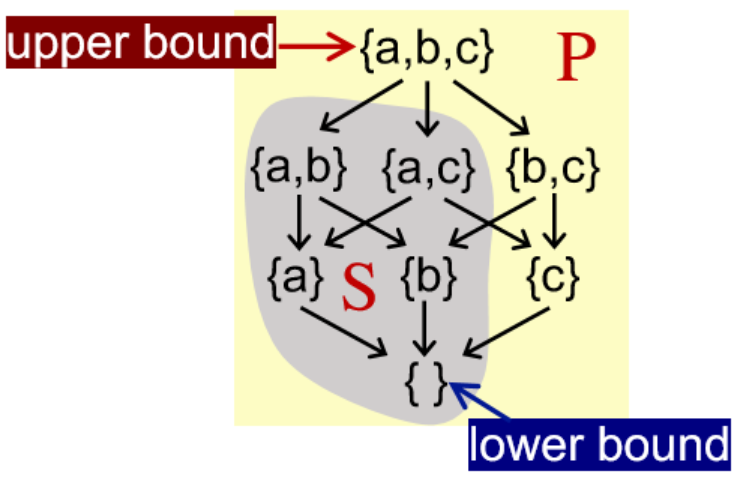
\includegraphics{img/upper_bound.png}

\subsection{最小上界、最大下界}
We define the least upper bound (lub or join) of $S$, written $\sqcup S$, if for every upper bound
of $S_{1}$ say $u, \sqcup S \sqsubseteq u$. Similarly, We define the greatest lower bound (glb or meet) of $S$,
written $\sqcap S_{,}$ if for every lower bound of $S$, say $l, l \sqsubseteq \sqcap S$.

$\text { 特别的, 对于仅有两个元素的集合 } S=\{a, b\}, \sqcup S \text { 可以写为 } a \sqcup b \text { , 同理 } \sqcap S \text { 可以写为 } a \sqcap b \text { 。 }$

注意:(最小)上界和(最大)下界是针对集合中的特定子集的,而上下界本身不一定在子集中,并且:
\begin{enumerate}
  \item 不是所有偏序集均存在lub或者glb(如先前灰色的集合就不含lub)
  \item 如果一个偏序集存在lub和glb,那么它是唯一的\\
  证明: 设$g1$ 和$g2$ 同为 $P$ 的glb,那么根据定义 $g_1\sqsubseteq(g_2=\sqcap P)$ 并且$g_2\sqsubseteq(g_1=\sqcap P)$,又因为反对称性,所以$g_1=g_2$
  \end{enumerate}

\section{Lattice, Semilattice, Complete and Product Lattice}
\subsection{Lattice(格)}
Given a poset $(P, \sqsubseteq), \forall a, b \in P$, if $a \sqcup b$ and $a \sqcap b$ exist, then $(P, \sqsubseteq)$ is called a lattice.

如果一个偏序集的任意两个元素都有最小上界和最大下界,那么这一偏序集是一个\textbf{格}

\subsection{Semilattice}
最小上界和最大下界只存在一个的偏序集称\textbf{半格},只存在最小上界称为“join semilattice”,只存在最大下界称为“meet semilattice”。

\subsection{Complete Lattice}
Given a lattice $(P, \sqsubseteq)$, for arbitrary subset $S$ of $P$, if $\sqcup S$ and $\sqcap S$ exist, then $(P, \sqsubseteq)$ is
called a complete lattice.

一个偏序集的任意子集均存在最小上界和最大下界,那么这个偏序集成为全格。
每个全格都存在一个最大元素 top $(\top=\sqcup P)$ 和最小元素bottom $(\perp=\sqcap P)$
所有元素有限的格 (finite lattice) 均是全格。 (反之不成立)
\subsection{Product Lattice}
Given lattices $\left.L_{1}=\left(P_{1}, \sqsubseteq_{1}\right), L_{2}=\left(P_{2}, \sqsubseteq_{2}\right), \ldots, L_{n}=\left(P_{n}, \sqsubseteq\right) n\right)$, if for all $i,\left(P_{i}, \sqsubseteq_{i}\right)$
has $\sqcup i$ (least upper bound) and $\Pi_{i}$ (greatest lower bound), then we can have a product
lattice $L^{n}=(P, \sqsubseteq)$ that is defined by:
\begin{enumerate}
\item $P=P_{1} \times \ldots \times P_{n}$
\item $\left(x_{1}, \ldots, x_{n}\right) \sqsubseteq\left(y_{1}, \ldots, y_{n}\right) \Leftrightarrow\left(x_{1} \sqsubseteq y_{1}\right) \wedge \ldots \wedge\left(x_{n} \sqsubseteq y_{n}\right)$
\item $\left(x_{1}, \ldots, x_{n}\right) \sqcup\left(y_{1}, \ldots, y_{n}\right)=\left(x_{1} \sqcup_{1} y_{1}, \ldots, x_{n} \cup_{n} y_{n}\right)$
\item  $\left(x_{1}, \ldots, x_{n}\right) \sqcap\left(y_{1}, \ldots, y_{n}\right)=\left(x_{1} \sqcap_{1} y_{1}, \ldots, x_{n} \sqcap_{n} y_{n}\right)$
\end{enumerate}
Product Lattice仍是Lattice, 若每个子格为全格,那么乘积也是全格。
\subsection{Data Flow Analysis Framework via Lattice}
一个数据流分析框架可以表示为一个三元组 $(D, L, F)$, 其中:
\begin{enumerate}
\item D: 指数据流分析的方向, i.e., forward or backward;
\item $\mathrm{L}$ : 指lattice, 该格表示所有domain值域, 以及meet (П) 或join $(\sqcup)$ 操作;
\item F: 一组transfer function.
\end{enumerate}

\section{Monotonicity and Fixed Point Theorem}
Monotonicity 
A function $f: L \rightarrow L(L$ is a lattice) is monotonic if $\forall x, y \in L, x \sqsubseteq y \Longrightarrow f(x) \sqsubseteq f(y)$
普通函数的单调性的推广
\subsection{Fixed-Point Theorem}
Given a complete lattice $(L, \sqsubseteq)$, if (1) $f: L \rightarrow L$ is monotonic and (2) $L$ is finite, then the least fixed point of $f$ can be found by iterating $f(\perp), f(f(\perp)), \ldots, f^{k}(\perp)$ until a fixed
point is reached the greatest fixed point of $f$ can be found by iterating
$f(\top), f(f(\top)), \ldots, f^{k}(T)$ until a fixed point is reached.\\
如果番调且L有界, 那么荐在不动点, 从上开始迭代执行 $f$ 可得最小不动点, 从丁开始迭代可得最大不动
点。\\
\textbf{证明:}\\
(1) Existence
由上定义以及 $f: L \rightarrow L$ 可楊
$$
\perp \sqsubseteq f(\perp)
$$
又因 $f$ 是单调的,因此
$$
f(\perp) \sqsubseteq f(f(\perp))=f^{2}(\perp)
$$
由于L是有限(finite)的, 因此总会存在一个 $k$, 有
$$
f^{F i x}=f^{k}(\perp)=f^{k+1}(\perp)
$$
(2) Least Fixed Point (数归法, 证明最小)
假设我们有另一个不动点x, i.e., $x=f(x)$(单调性)
由上的定义, 我们有$\perp\sqsubseteq x_{i}$
下面用数归法证明:\\
由于 $f$ 是单调的,因此
$$
f(\perp) \sqsubseteq f(x)
$$
对于 $f^{i}(\perp) \sqsubseteq f^{i}(x)$, 由于 $f$ 是单调的, 因此有
$$
f^{i+1}(\perp) \sqsubseteq f^{i+1}(x)
$$
因此对于任意i, 有
$$
f^{i}(\perp) \sqsubseteq f^{i}(x)
$$
又因为 $x=f(x)$, 所以存在一个i, 有 $f^{i}(\perp) \sqsubseteq f^{i}(x)=x$, 因此有
$$
f^{F i x}=f^{k}(\perp) \sqsubseteq x
$$
因此 $f^{i}(\perp)$ 是最小不动点。

\section{Relate lterative Algorithm to Fixed Point Theorem}
如何将迭代算法和不动点定理联系起来?
\begin{enumerate}
  \item 程序中每一个状态为一个product lattice
  \item Transfer function和join/meet fucntion可以视为F
\end{enumerate}

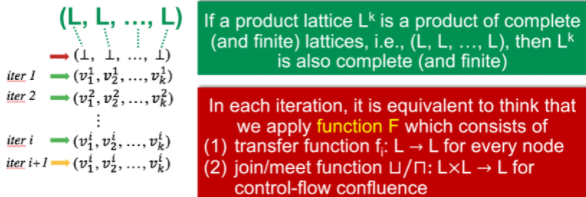
\includegraphics{img/lattice.png}

下面只需要证明Transfer function和 join/meet function均为单调的即可

\begin{enumerate}
\item Transfer function是单调的, 因为通过之前分析,所有Gen/Kill的函数都是单
调的;
\item Join/meet function是单调的, 证明如下
\end{enumerate}
要证Join/meet function,就是要证
$$\forall x, y, z \in L, x \sqsubseteq y \rightarrow x \sqcup z \sqsubseteq - y \sqcup z$$
由 $\sqcup$ 定义可得, $y \sqsubseteq y \sqcup z$,
由于巨传递性, $x \sqsubseteq y$, 因此 $x \sqsubseteq y \sqcup z$, 因此 $y \sqcup z$ 是 $x$ 的上界,
注意到 $y \sqcup z$ 也是 $z$ 的上界, 而 $x \sqcup z$ 是 $x$ 和 $z$ 的最小上界,
因此 $x \sqsubseteq y \Rightarrow x \sqcup z \sqsubseteq y \sqcup z$

\subsection{讨论算法复杂度}
定义格的高度即从top至bottom的最长路径长,
The height of a lattice $h$ is the length of the longest path from Top to
Bottom in the lattice.
最坏情况即一次迭代,只变化一个单位高度,因此复杂度为 $O(h \times k) .$

\section{May/Must Analysis, A Lattice View*}
任何分析初始状态都从unsafe至safe。针对于分析结果而言,处理所有分析结果后,程序行为正常为safe,反之为unsafe,极端的safe是无用的(如安全扫描中的模式匹配)

Must和May分析的示意图如下图所示,对于Must分析,每个代码块都是从$\top$开始的,因为在程序一开始,算法认为所有的待分析对象都是“合格”的(例如存活表达式分析中,算法认为每个表达式都是成活的)——这是一个不安全的状态,经过不断迭代,算法逐渐下降到最大不动点,虽然已经过了truth点(漏报),但是这已经是最好情况了(越往下走越safe但是结果也没意义了),对这些结果做优化能确保程序不出错(safe)。

对于May分析,每个代码块从$\perp$开始,即在一开始,算法认为所有分析对象都是不合格的(例如定义可达性分析中,算法认为每一条定义都没有新的定义)——这是May类型的不安全状态,经过不断迭代,算法逐渐上升到最小不动点,同样也过了truth(误报),这也是分析的最好情况,算法依旧停留在safe区域。
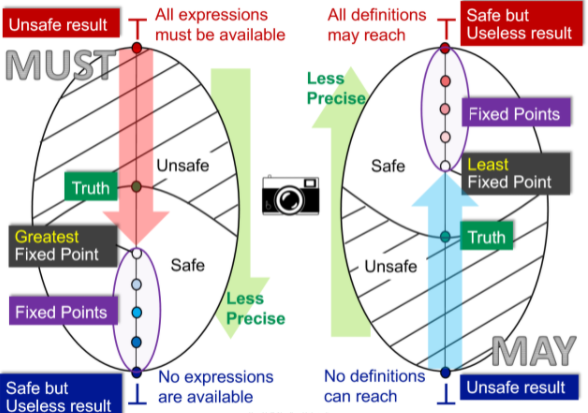
\includegraphics{img/must.png}

\section{Distributivity(分配性) and MOP}
\subsection{MOP(Meet-Over-All-Paths Solution)}
设 $s_{x}$ 为矢 设 $F_{p}$ 是一个路径 $P$ 上的 transfer function, 那么 $\operatorname{MOP}\left[S_{i}\right]=\sqcup / \sqcap_{\mathrm{A} \text { path } P \text { from Entry to } S_{i}} F_{p}(O U T[E n t r y])$
\\
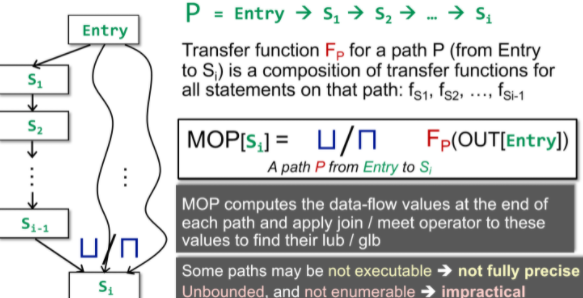
\includegraphics{img/moap.png}\\
就是说,之前数据流分析的结果是流敏感的, 而 MOP 的结果是路径敏感的,
例 如 下 图 所 示 的 数 据 流,,数 据 流 分 析 的 结 果 是
$\mathrm{IN}\left[\mathrm{s}_{4}\right]=f_{s_{3}}\left(f_{s_{1}}(\mathrm{OUT}[\right.$ entry $]) \sqcup f_{S_{2}}($ OUT $[$ Entry $\left.])\right)$, 而 MOP 是
$\operatorname{MOP}\left[\mathrm{s}_{4}\right]=f_{S_{3}}\left(f_{s_{1}}(\mathrm{OUT}[\right.$ entry $\left.])\right) \sqcup f_{S_{3}}\left(f_{S_{2}}(\mathrm{OUT}[\right.$ Entry $\left.])\right)\left(\right.$ 注意 $f_{s_{3}}$
的位置)\\
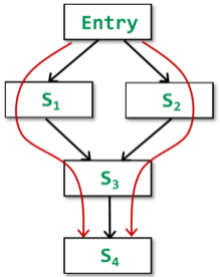
\includegraphics{img/mop.png}
\subsection{Iterative Algorithm v.s. MOP}
MOP比Iterative分析更精确,也就是说路径敏感比敏感更精确,下面为证明(这里只需证明两条路径的情况,其它数归即可):


然而,当F是distributive(F满足分配率)时,Interative和MOP一样准确。

BitVector或是Gen/Kill问题(set union/intersection for join/meet)都是满足分配率的

\subsection{Constant Propagation}

Given a variable x at program point p, determine whether x is guaranteed to hold a constant value at p
对于在程序点 p 的一个变量 x,判断 x 是否为在 p 点为一个常量

分析结果:对于每一个CFG节点,对应一个 (x,v) 集合,x 是变量,v 是 x 的值
\subsection{Lattice}
Domain: UNDEF $\rightarrow\{\ldots,-2,-1,0,1,2, \ldots\} \rightarrow \mathrm{NAC}, \rightarrow$ 表示 $\sqsubseteq$ 关系
Meet Operator $\sqcup$:
\begin{enumerate}
   
  \item $\mathrm{NAC} \sqcap v=\mathrm{NAC}$
  \item $UNDEF \sqcap v=v$
  \item $c \sqcap v=\mathrm{NAC} \quad(\mathrm{c}$ 为一常量)
  \item $c \sqcap c=c$
  \item $c_{1} \sqcap c_{2}=\mathrm{NAC}$
\end{enumerate}

\subsection{Transfer Function}
讨论transfer function, 对于一个赋值语句 $\mathrm{s}: \mathrm{x}=\ldots$ 来说, 定义其 $\mathrm{F}$ 为
$$
F: \operatorname{OUT}[s]=\operatorname{gen} \cup\left(\operatorname{IN}[s]-\left\{\left(x,_{-}\right)\right\}\right)
$$
- $\mathrm{s}: \mathrm{x}=\mathrm{c} ;$ gen $=\{(x, c)\}$
व-s: $\mathrm{x}=\mathrm{y} ;$ gen $=\{(x, \operatorname{val}(y))\}$
- s: $x=y$ op z; gen $=\{(x, f(x, z))\}$
而 $f(x, z)$ 有三种情况:
$$
f(y, z)=\left\{\begin{array}{ll}
\operatorname{val}(y) \text { op } \operatorname{val}(z) & / / \text { if } \operatorname{val}(\mathrm{y}) \text { and } \operatorname{val}(\mathrm{z}) \text { are constants } \\
\mathrm{NAC} & / / \text { if } \operatorname{val}(\mathrm{y}) \text { or } \mathrm{val}(\mathrm{z}) \text { is } \mathrm{NAC} \\
\mathrm{UNDEF} & / / \text { otherwise }
\end{array}\right.
$$
\subsection{function不满足分配性}
如下图所示,$F(X \sqcap Y)$ 中C的值为NAC,而$F(X) \sqcap F(Y)$中 C 的值为10,因此F不满足分配性。
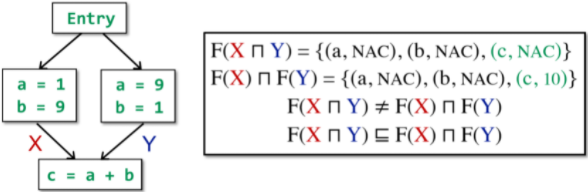
\includegraphics{img/distrib.png}
\section{Worklist Algorithm}
Iterative Algorithm的优化,Iterative 存在冗余的计算,而Worklist只计算有变化的node:
\begin{lstlisting}
OUT[entry] =∅;
for(each basic block B\entry) 
	OUT[B] =∅;
    Worklist←all basic blocks
	while (Worklist is notempty) 
    	Pick a basic block B from Worklist
		old_OUT= OUT[B]
        IN[B] =⊔OUT[P]; # join/meet P为B的前置代码块
        OUT[B] = genB U (IN[B] - killB); # transfer function 
        if(old_OUT≠OUT[B])
        	Add all successors of B to Worklis
\end{lstlisting}

\subsection{分析特性}
\begin{enumerate}
  \item 流敏感:程序语句随意调换位置,分析结果不变为流非敏感,否则为流敏感;
  \item 路径敏感:考虑程序中路径的可行性;
\end{enumerate}
\section{Space of dataflow ananlys \cite{cs153lec18}}
$$\begin{array}{|c|c|c|}
  \hline & \text { May } & \text { Must } \\
  \hline \text { Forward } & \begin{array}{c}
  \text { Reaching } \\
  \text { definitions }
  \end{array} & \begin{array}{c}
  \text { Available } \\
  \text { expressions }
  \end{array} \\
  \hline \text { Backward } & \text { Live variables } & \begin{array}{c}
  \text { Very busy } \\
  \text { expressions }
  \end{array} \\
  \hline
  \end{array}$$
 \subsection{Available Expressions}
 \begin{enumerate}
     \item An expression e is available at program point $p$ if on all paths from the entry to $p$, expression e is computed at least once, and there are no intervening  assignment to $\mathrm{x}$ or to the free variables of $\mathrm{e}$
     \item If e is available at $p$, we do not need to re-compute e
     
\begin{enumerate}
    \item (i.e., for common sub-expression elimination)
\end{enumerate}
\item How do we compute the available expressions at each program point?
 \end{enumerate}
 \begin{figure}[htbp]
  \centering
  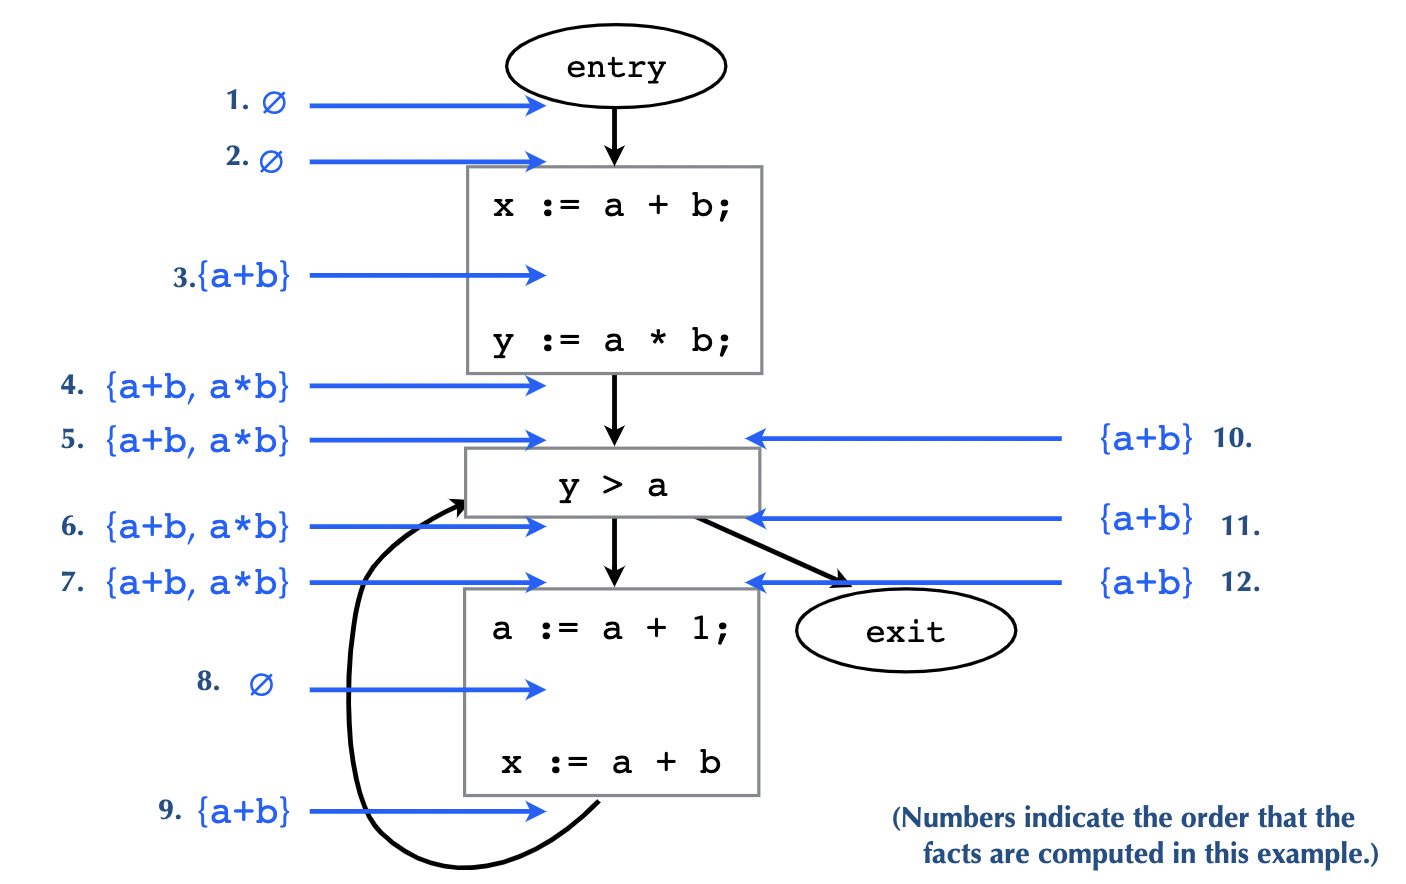
\includegraphics[width=10cm]{./img/avail.png}
\end{figure}
Formally:
\begin{enumerate}
    \item Suppose $D$ is a set of expressions that are available at program point $p$
\item Suppose $p$ is immediately before " $\mathrm{x}:=\mathrm{e}_{1} ; \quad \mathrm{B}^{\prime \prime}$
\item Then the statement " $\mathrm{x}:=\mathrm{e}_{1}$ "
\begin{enumerate}
    \item generates the available expression $\mathbf{e}_{1}$
    \item kills any available expression $\mathbf{e}_{2}$ in $D$ such that $\mathbf{x}$ is in variables $\left(\mathbf{e}_{2}\right)$
    
\end{enumerate}
\item So the available expressions for B are: $\left(D \cup\left\{\mathbf{e}_{1}\right\}\right)-\left\{\mathbf{e}_{2} \mid \mathbf{x} \in \operatorname{variables}\left(\mathbf{e}_{2}\right)\right\}$
\end{enumerate}

$$\begin{array}{|c|c|c|}
\hline \text { Stmt } & \text { Gen } & \text { Kill } \\
\hline \mathbf{x}:=\mathbf{v} & \{\mathrm{v}\} & \{\mathrm{e} \mid \mathrm{x} \text { in } \mathrm{e}\} \\
\hline \mathbf{x}:=\mathbf{v}_{1} \text { op } \mathbf{v}_{2} & \left\{\mathbf{v}_{1} \text { op } \mathrm{v}_{2}\right\} & \{\mathrm{e} \mid \mathrm{x} \text { in } \mathrm{e}\} \\
\hline \mathbf{x}:=*(\mathrm{v}+i) & \{\} & \{\mathrm{e} \mid \mathrm{x} \text { in } \mathrm{e}\} \\
\hline *(\mathrm{v}+i):=\mathrm{x} & \{\} & \{\} \\
\hline \text { jump } \mathrm{L} & \{\} & \{\} \\
\hline \text { return } \mathrm{v} & \{\} & \{\} \\
\hline \text { if v1 op v2 goto I1 else goto L2 } & \{\} & \{\} \\
\hline \mathbf{x}:=\mathbf{v}\left(\mathbf{v}_{1}, \ldots \mathbf{v}_{\mathrm{n}}\right) & \{\} & \{\mathrm{e} \mid \text { in } \mathrm{e}\} \\
\hline
\end{array}$$

$$\text { Transfer function for stmt } S: \lambda D .\left(D \cup G e n_{S}\right)-\text { Kill }_{S}$$
\subsubsection{Aliasing}
You can use Aliasing to save register!
\begin{enumerate}
    \item We can tell whether variables names are equal.
\item We cannot (in general) tell whether two variables will have the same value.
\item If we track * $\mathrm{x}$ as an available expression, and then see $* y:=e^{\prime}$, don't know whether to kill * $x$
\item Don't know whether x's value will be the same as $y^{\prime}$ s value
\end{enumerate}
\begin{minted}[mathescape,linenos]{c}
void accumulate_restrict(int* restrict source, int len, int* restrict target) {
    for (int i = 0; i < len; i++) {
        *target += source[i];
    }
}
\end{minted}
\subsection{Reaching Definitions}
\begin{enumerate}
    \item A definition $\mathrm{x}:=\mathrm{e}$ reaches a program point $p$ if there is some path from the assignment to $p$ that contains no other assignment to $\mathrm{x}$
\item Reaching definitions useful in several optimizations, including constant propagation
\item Can also define reaching definitions analysis using gen and kill sets; combine dataflow facts at merge points by union
\end{enumerate}
Define $\operatorname{defs}(\mathbf{x})$ to be the set of all definitions of variable $x$
$$\begin{array}{|c|c|c|}
\hline \text { Stmt } & \text { Gen } & \text { Kill } \\
\hline \mathrm{d}: \mathbf{x}:=\mathbf{v} & \{\mathrm{d}\} & \operatorname{defs}(\mathbf{x})-\{\mathrm{d}\} \\
\hline \mathrm{d}: \mathbf{x}:=\mathbf{v}_{1} \text { op } \mathbf{v}_{2} & \{\mathrm{~d}\} & \operatorname{defs}(\mathbf{x})-\{\mathrm{d}\} \\
\hline \text { everything else } &  &  \\
\hline
\end{array}$$
\begin{enumerate}
    \item $$
D_{\text {in }}[\mathrm{L}]=\cup\left\{D_{\text {out }}\left[\mathrm{L}^{\prime}\right] \mid \mathrm{L}^{\prime} \text { in pred }[\mathrm{L}]\right\}
$$
\item Transfer function for stmt $S: \lambda D$. (D $\cup \mathrm{Gen} s)-\mathrm{Kill}_{S}$
\end{enumerate}
\subsection{Liveness}
\begin{enumerate}
    \item  Variable $\mathbf{x}$ is live at program point $p$ is there is a path from $p$ to a use of variable $\mathrm{x}$
\item Liveness useful in dead code elimination and register allocation
\item Can also define using gen-kill sets
\item However, we use a backward dataflow analysis i.e., instead of flowing facts forwards over statement (computing $D_{\text {out }}$ from $D_{\text {in }}$ ) we flow facts backwards over statements (compute $D_{\text {in }}$ from $D_{\text {out }}$ )
\end{enumerate}
$$\begin{array}{|c|c|c|}
\hline \text { Stmt } & \text { Gen } & \text { Kill } \\
\hline \mathbf{x}:=\mathbf{v} & \{\mathbf{v} \mid \text { if } \mathrm{v} \text { is variable }\} & \{\mathbf{x}\} \\
\hline \mathbf{x}:=\mathbf{v}_{1} \text { op } \mathbf{v}_{2} & \left\{\mathrm{v}_{i} \mid i \in 1,2, \mathrm{v}_{i} \text { is var }\right\} & \{\mathbf{x}\} \\
\hline \mathbf{x}:=*(\mathrm{v}+i) & \{\mathbf{v} \mid \text { if } \mathrm{v} \text { is variable }\} & \{\mathbf{x}\} \\
\hline *(\mathrm{v}+i):=\mathbf{x} & \{\mathrm{x}\} \cup\{\mathrm{v} \mid \text { if } \mathrm{v} \text { is variable }\} & \{\} \\
\hline \text { jump L } & \{\} & \{\} \\
\hline \text { return } \mathrm{v} & \{\mathrm{v} \mid \text { if } \mathrm{v} \text { is variable }\} & \{\} \\
\hline \text { if } \mathrm{v}_{1} \text { op v2 goto L1 else goto L2 } & \left\{\mathbf{v}_{i} \mid i \in 1,2, \mathbf{v}_{i} \text { is var }\right\} & \{\} \\
\hline \mathbf{x}:=\mathbf{v}_{0}\left(\mathrm{v}_{1}, \ldots \mathrm{v}_{\mathrm{n}}\right) & \left\{\mathbf{v}_{i} \mid i \in 0 . . n, \mathrm{v}_{i} \text { is var }\right\} & \{\mathrm{x}\} \\
\hline
\end{array}$$
\begin{enumerate}
    \item i.e., any use of a variable generates liveness, any definition kills liveness 
    \item $D_{\text {out }}[\mathrm{L}]=\cup\left\{D_{\text {in }}\left[\mathrm{L}^{\prime}\right] \mid \mathrm{L}^{\prime}\right.$ in $\left.\operatorname{succ}[\mathrm{L}]\right\}$
    \item $$\text { Transfer function for stmt } S: \lambda D .\left(D \cup \text { Gen }_{S}\right)-\text { Kill }_{S}$$
\end{enumerate}
\begin{figure}[htbp]
  \centering
  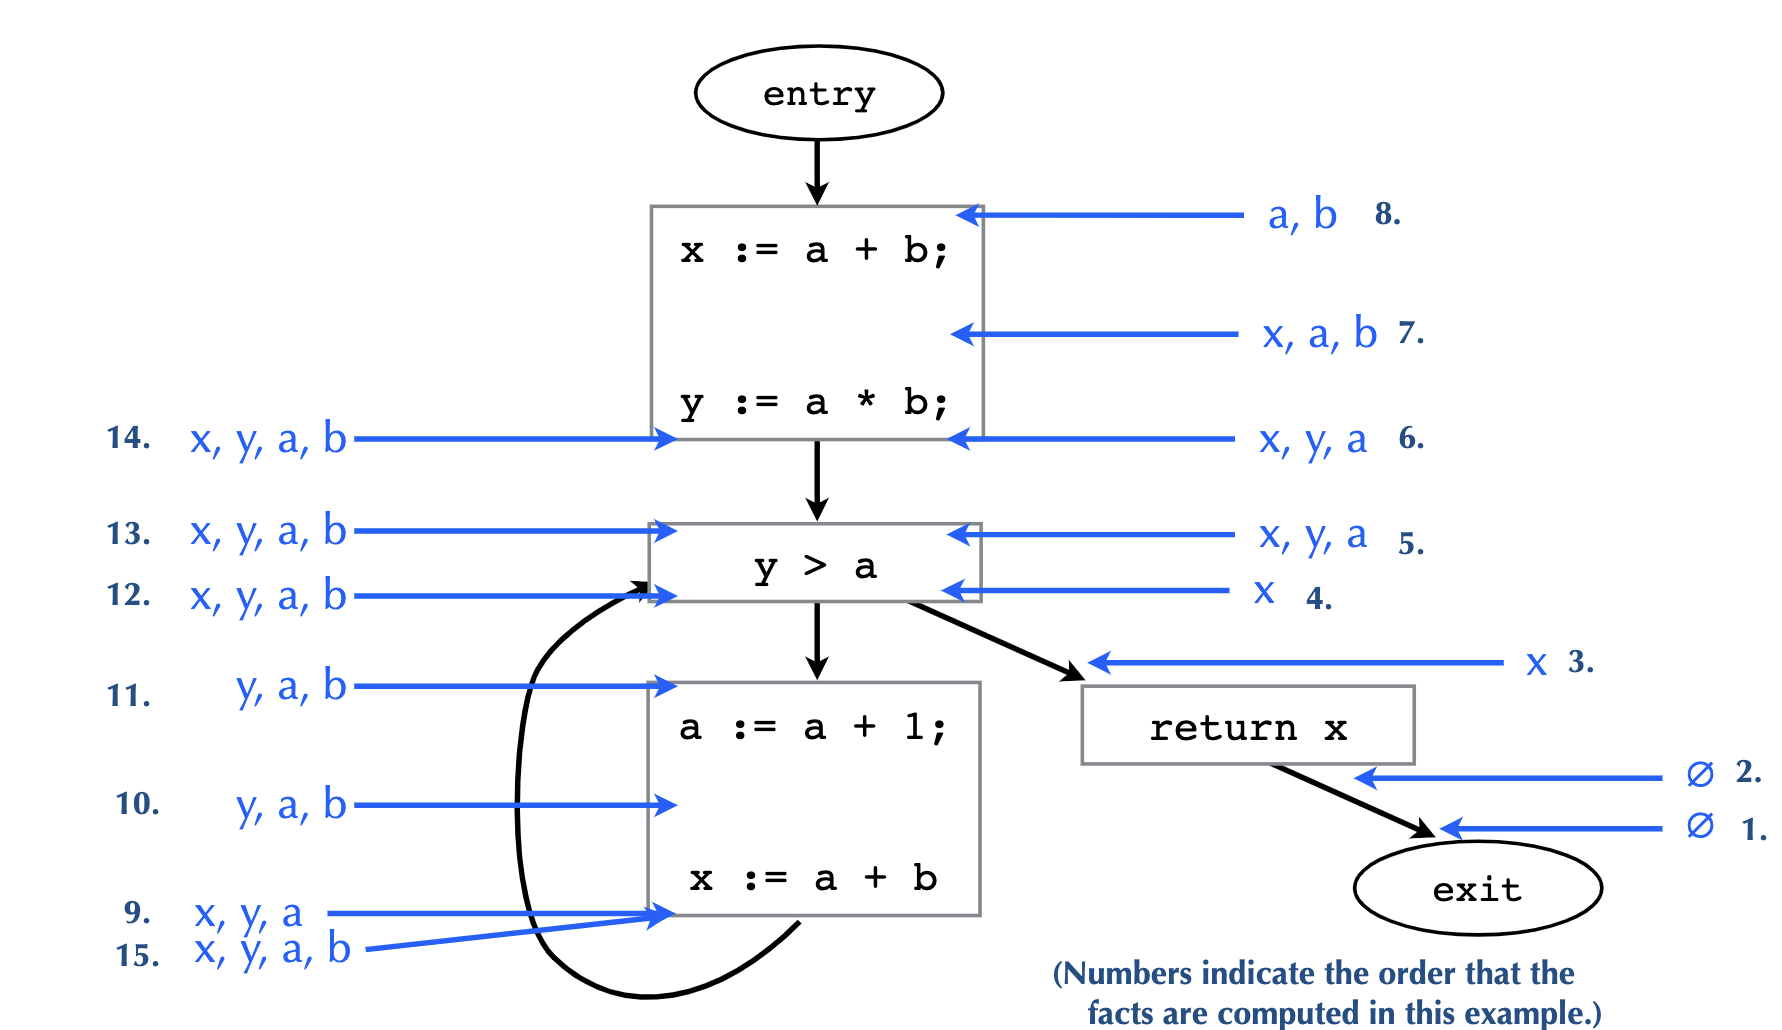
\includegraphics[width=10cm]{./img/liveness.png}
\end{figure}
\printbibliography
\end{document}
